\setstretch{1.000}
\section{Auswertung}

Im folgenden werden Energieverlust und Winkelabhängigkeit der an Goldfolie gestreuten Alphateilchen untersucht. Die Berechnung der Werte
erfolgt unter Verwendung der Python \cite{python} Pakete NumPy \cite{numpy} und SciPy \cite{scipy} sowie Uncertainties \cite{uncertainties} zur
Unsicherheitsfortpflanzung in erster Ordnung. Grafiken werden mithilfe von Matplotlib \cite{matplotlib} generiert. Zunächst können einige
weiterhin benötigten Größen bestimmt werden.

\subsection*{Vorbereitung}

Mit einer Aktivität von $\qty{330}{\kilo\becquerel}$ im Oktober $1994$ und einer Halbwertszeit von $432.2 \: \text{yr}$~\cite{Americium_2004}
ergibt sich wie in Abbildung \ref{fig:Aktivität} dargestellt nach $30$ Jahren eine erwartete Zerfallsrate von $\qty{314.5}{\kilo\becquerel}$
für die verwendete $\ce{^{241}_{95}Am}$ Probe.

% Um die gesuchten Werte und Messgrößen zu bestimmen, ist es notwendig, im Vorfeld einige wichtige Größen zu berechnen und festzuhalten.  
% Die Aktivität des verwendeten Isotops $^{241}\mathrm{Am}$ wird für das Jahr 1994 mit \SI{330}{\kilo \becquerel} angegeben.  
% Unter Berücksichtigung der Halbwertszeit von Americium ergibt sich für das Jahr 2024 eine Aktivität von \SI{314.5}{\kilo \becquerel}.  
% Ein graphischer Verlauf der Aktivität ist in \autoref{fig:Aktivität} dargestellt.

\begin{figure}[H]
    \centering
    \includegraphics[width=0.963\textwidth]{content/messung/Aktivität.pdf}
    \caption{Graphischer Verlauf der Aktivität von $\ce{^{241}Am}$ über die Zeit.}
    \label{fig:Aktivität}
\end{figure}

Außerdem sollten die Kernladungszahlen und Teilchenzahldichten $N$ von Luft und Gold bestimmt werden, um diese in \eqref{eqn:Bethe} einsetzen
zu können. Dazu wird genähert, dass die Anteile $\qty{78}{\percent}$ und $\qty{21}{\percent}$ von Stickstoff und Sauerstoff die vollständige
Zusammensetzung von Luft beschreiben. Aus $Z_{N_2} = 7$ und $Z_{O_2} = 8$ folgt demnach
$Z_L = \tfrac{78}{99} Z_{N_2} + \tfrac{21}{99} Z_{O_2} = \num{7.21}$ als mittlere Kernladungszahl. Analog ergeben sich die molare
Masse $M_L = \qty{28.86}{\gram\per\mole}$ sowie $\rho_L = \qty{1200}{\gram\per\meter\cubed}$ für die Dichte. Gold hat $Z_G = 79$ sowie
$M_G = \qty{196.67}{\gram\per\mole}$ und $\rho_G = \qty{19.32e6}{\gram\per\meter\cubed}$ bei Raumtemperatur \cite{Greenwood_1998}.

% Des Weiteren ist es hilfreich, die Teilchenzahl und Dichte von Luft und Gold vorab zu bestimmen.  
% Da Atemluft hauptsächlich aus Stickstoff und Sauerstoff besteht, können die mittlere Kernladungszahl, die molare Masse und die Dichte der Luft  
% durch die Eigenschaften von Stickstoff und Sauerstoff wie folgt ausgedrückt werden:

Die Teilchendichten lassen sich nun über den Zusammenhang
\begin{equation*}
	N = N_{\! A} \frac{\rho}{M}
\end{equation*}
zu $N_L = \qty{2.5e25}{\per\meter\cubed}$ und $N_G = \qty{5.9e28}{\per\meter\cubed}$ bestimmen. Für Alphateilchen gilt noch $z = 2$ als
Kernladungszahl, um deren Reichweite abschätzen zu können.

% \begin{align*}
% Z_{N_2} &= 7, & Z_{O_2} &= 8, & Z_L &= \frac{78}{99} Z_{N_2} + \frac{21}{99} Z_{O_2} = 7.21, \\
% M_{N_2} &= 2 \cdot 14.01 \, \text{g/mol}, & M_{O_2} &= 2 \cdot 16.00 \, \text{g/mol}, & M_L &= \frac{78}{99} M_{N_2} + \frac{21}{99} M_{O_2} = 28.86 \, \text{g/mol}, \\
% \rho_{N_2} &= 1165 \, \text{g/m}^3, & \rho_{O_2} &= 1332 \, \text{g/m}^3, & \rho_L &= \frac{78}{99} \rho_{N_2} + \frac{21}{99} \rho_{O_2} = 1200 \, \text{g/m}^3.
% \end{align*}
% 
% Die Dichte und die molare Masse von Gold sind gegeben durch:
% 
% \begin{align*}
% M_G &= 196.67 \, \text{g/mol}, & \rho_G &= 19320 \, \text{kg/m}^3.
% \end{align*}
% 
% Hierüber lassen sich die Teilchendichten von Luft und Gold berechnen:
% 
% \begin{align*}
% N_L &= N_A \frac{\rho_L}{M_L} = 250 \cdot 10^{23} \, \text{m}^{-3}, \\
% N_G &= N_A \frac{\rho_G}{M_G} = 591000 \cdot 10^{23} \, \text{m}^{-3}.
% \end{align*}

% Die druckabhängige Reichweite der $\alpha$-Strahlung ist gegeben durch:
% 
% \[
% \rho = \frac{p}{RT}, \qquad R_\alpha \propto p^{-1}.
% \]
% 
% Für den Zerfall von $^{241}\text{Am}$ gilt
% 
% \[
% ^{241}_{95}\text{Am} \rightarrow ^{237}_{93}\text{Np} + ^4_2\text{He} + E_\alpha, \qquad E_\alpha = 5.486 \, \text{MeV}.
% \]

\subsection*{Reichweite}

Zur Ermittlung der Reichweite muss \eqref{eqn:Bethe} umgestellt und nach
\begin{equation*}
	R_\alpha = \, -\!\int_{\: 0}^{E_\alpha} \!\! \pfrac{dE}{dE / dx}
\end{equation*}
integriert werden. Dazu besitzt der Heliumkern im Prozess
\begin{equation*}
	\ce{^{241}_{95}Am} \longrightarrow \ce{^{237}_{93}Np} + \ce{^4_2He} + E_\alpha
\end{equation*}
bei der häufigsten Zerfallsmode $E_\alpha = \qty{5.486}{\mega\electronvolt}$ \cite{Americium_2004}. Numerische Integration liefert
dann eine Reichweite $R_\alpha = \qty{6.9}{\centi\meter}$ in Luft. Zum Vergleich können die Werte $\qty{0.5}{\centi\meter}$ und
$\qty{9.5}{\centi\meter}$ als Reichweiten für Energien von $\qty{1}{\mega\electronvolt}$ und $\qty{10}{\mega\electronvolt}$ aus
der Literatur \cite{Kolanoski_2007} entnommen werden, die unter Berücksichtigung relativistischer Korrekturterme berechnet wurden.

% \textbf{BETHE BLOCH THEORIE}

\subsection*{Foliendicke}

Der Energieverlust an der Goldfolie wird nun verwendet, um deren Dicke zu bestimmen. Dazu wird die maximale Pulshöhe unter Variation
des Kammerdruckes mit und ohne Folie im Strahlengang gemessen. Dieses Vorgehen beruht auf der Annahme, dass die emittierten Alphateilchen
einer symmetrischen Energieverteilung folgen. Ein höherer Druck sorgt dafür, dass nur noch Alphateilchen mit Energien größer oder gleich
einer entsprechenden Grenze den Detektor erreichen. Die Pulshöhe entspricht dann einer umgekehrten integrierten Verteilung wie
exemplarisch in Abbildung \ref{fig:Energieverteilung} gezeigt.

Ohne Folie gibt nun der Mittelwert $E_\alpha$ den Wendepunkt $p_\alpha$ an, in dessen Umgebung sich der Verlauf linear approximieren
lässt und der Wert genau der Hälfte des Maximums im abgeflachten Bereich geringer Drücke entspricht. Wird die Folie in den Strahlengang
positioniert, verschieben sich die Verteilungen um $\Delta p$ und es kann die dazu proportionale Energiedifferenz $\Delta E$ berechnet
werden. Als Formel ausgedrückt lässt sich also
\begin{equation*}
	\Delta E = E_\alpha \frac{\Delta p}{\raisebox{0.5ex}{$p_\alpha$}}
\end{equation*}
schreiben und nach Austauschen $dE / dx \longrightarrow \Delta E / \Delta x$ durch Umstellen von \eqref{eqn:Bethe} die Dicke $d = \Delta x$
berechnen. Die konkreten Messwerte dazu sind in Tabelle \ref{tab:Druck} aufgeführt.

\begin{table}[H]
	\centering
	\caption{Messdaten von Kammerdruck und maximaler Amplitude.}
	\label{tab:Druck}
	\hspace{9em}
	\begin{subfigure}{0.18\textwidth}
    	\centering
    	\caption{Ohne Folie.}
    	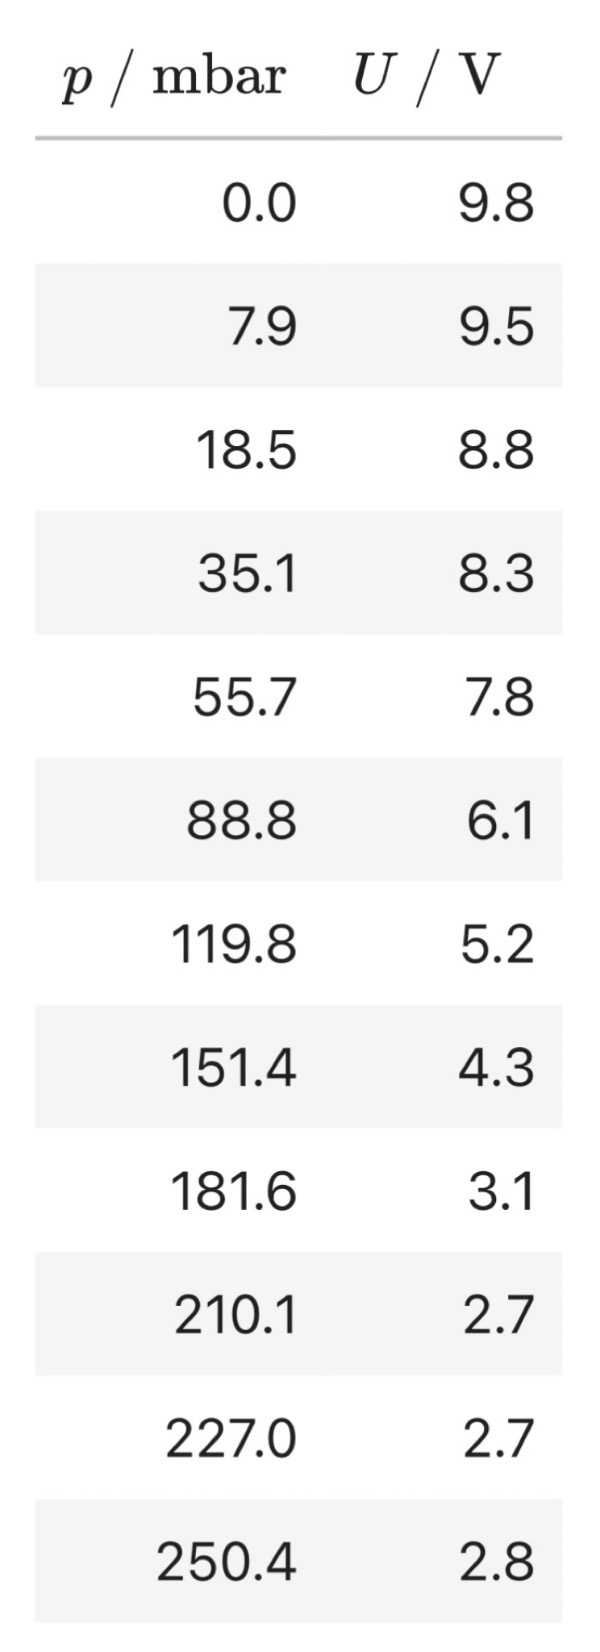
\includegraphics[width=\textwidth]{content/tabelle/OhneFolie.jpg}
    	\label{tab:OhneFolie}
	\end{subfigure}
	\hfill
	\begin{subfigure}{0.18\textwidth}
    	\centering
    	\caption{Mit Folie.}
    	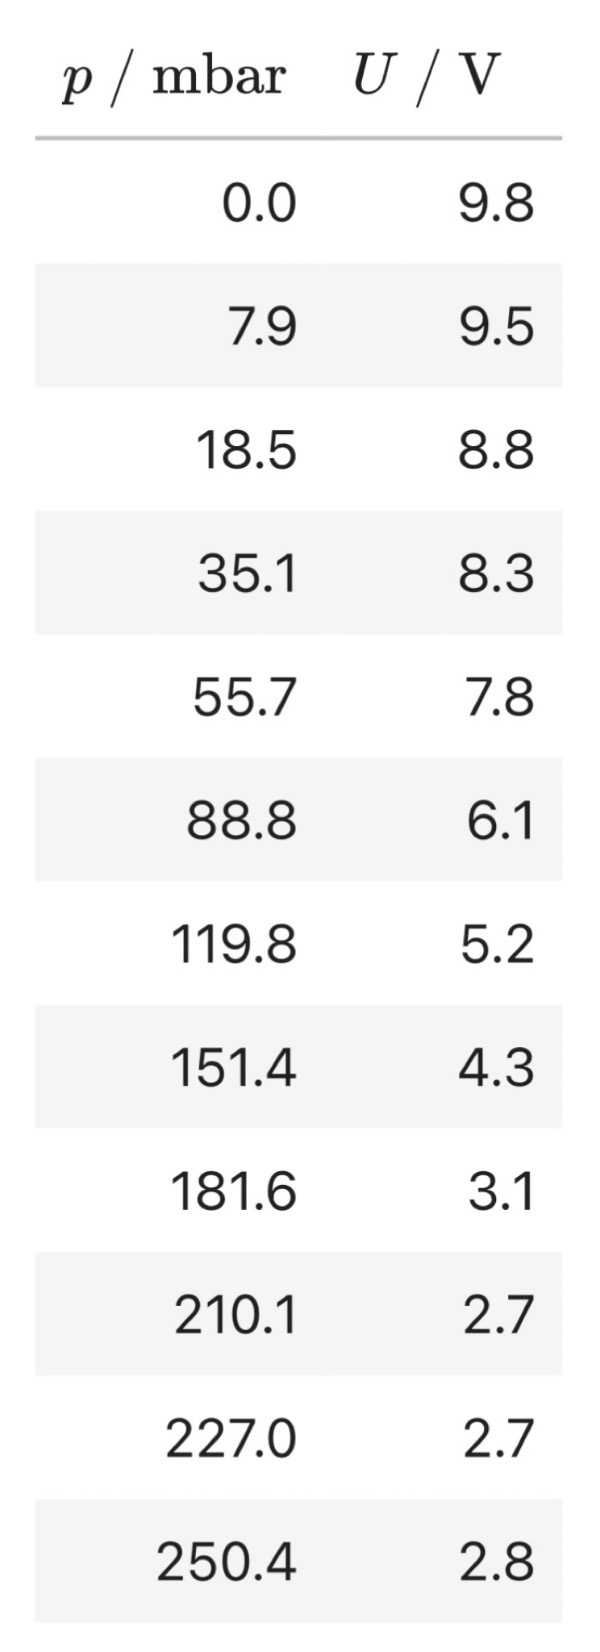
\includegraphics[width=\textwidth]{content/tabelle/MitFolie.jpg}
    	\label{tab:MitFolie}
	\end{subfigure}
	\hspace{9em}
\end{table}

\begin{figure}[H]
    \centering
    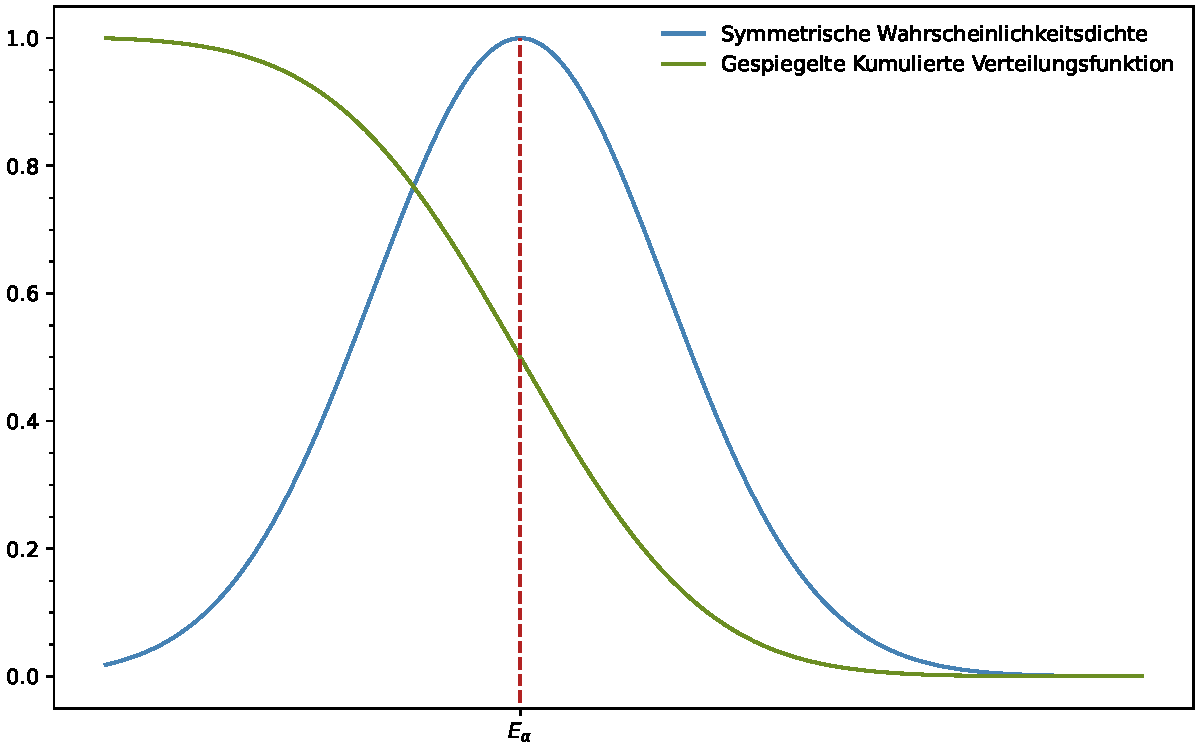
\includegraphics[width=0.963\textwidth]{content/messung/Energieverteilung.pdf}
    \caption{Normierte repräsentative Energieverteilungen der Alphastrahlung.}
    \label{fig:Energieverteilung}
\end{figure}

\begin{figure}[H]
    \centering
    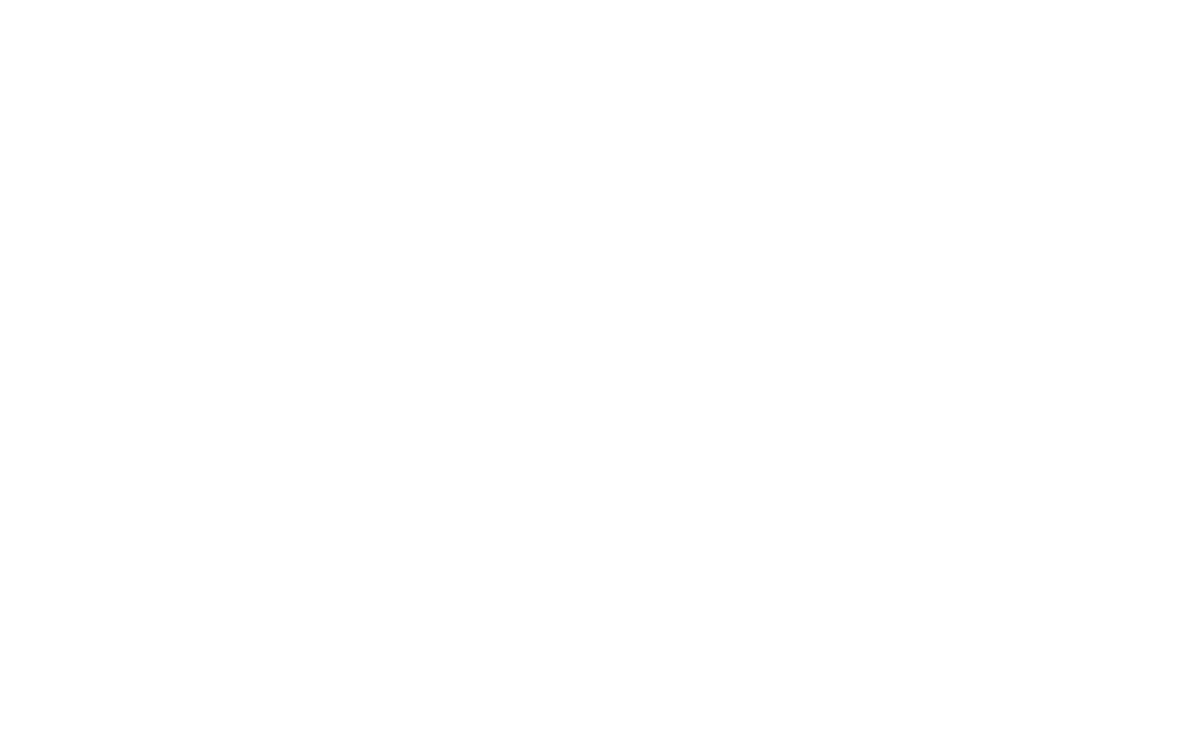
\includegraphics[width=\textwidth]{content/messung/Golddicke.pdf}
    \caption{Lineare Regressionen der Maximalspannungen $U$ in Abhängigkeit des Drucks $p$ mit und ohne Goldfolie.}
    \label{fig:Golddicke}
\end{figure}

Die in Abbildung \ref{fig:Golddicke} aufgetragenen Messwerte werden um die farblich hervorgehobenen Daten bei höheren Drücken wegen zu hohem
Rauschen bereinigt, um anschließend eine lineare Ausgleichsrechnung auszuführen. Die Funktion sowie die Umkehrung lauten also
\begin{align*}
	&&&& U = ap + b && \text{und} && p = \pfrac{U - b}{\raisebox{0.5ex}{$a$}} &&&&
\end{align*}
\vspace{-2em}
\begin{align*}
	& \text{mit} & a_\text{of} &= \qty{-0.0368+-0.0008}{\volt\per\milli\bar} &&
	\text{und} & b_\text{of} &= \qty{12.10+-0.12}{\volt} && \text{ohne Folie} \\
	& \text{sowie} & a_\text{mf} &= \qty{-0.0364+-0.0010}{\volt\per\milli\bar} &&
	\text{und} & b_\text{mf} &= \qty{9.65+-0.10}{\volt} && \text{mit Folie} \vspace{-2em}
\end{align*}
als Parameter aus der Regressionsrechnung. Damit und mit $U_\alpha = \qty{6.05}{\volt}$ ergeben sich $p_\alpha = \qty{165+-5}{\milli\bar}$
und $\Delta p = \qty{66+-6}{\milli\bar}$ sowie schließlich
\begin{equation*}
	\Delta E = \qty{2.2+-0.2}{\mega\electronvolt}
\end{equation*}
für die Energiedifferenz. Gleichung \eqref{eqn:Bethe} lässt sich dann zu
\begin{equation*}
	d = \Delta x = \Delta E \frac{4\pi m_e v_\alpha^2 \varepsilon_0^2}{e^4 N z^2 Z \ln (2m_e v_\alpha^2 / I)}
	= \Delta E \frac{8\pi m_e E_\alpha \varepsilon_0^2}{m_\alpha e^4 N z^2 Z \ln (4m_e E_\alpha / m_\alpha I)} =
	\qty{5.1+-0.4}{\micro\meter}
\end{equation*}
umstellen. Hier wird $I_G = Z_G \qty{10}{\electronvolt} = \qty{790}{\electronvolt}$ als Anregungspotential genähert.

% \subsection*{Bestimmung der Dicke der Goldfolie}
% 
% Die gemessenen Maximalspannungen in Abhängigkeit des Drucks wurden sowohl mit als auch ohne Goldfolie im Strahlengang aufgenommen.  
% Anschließend wurden lineare Regressionen durchgeführt. Die entsprechenden Graphen sind in \autoref{fig:Golddicke} dargestellt.
% 
% Die Parameter der Regressionsgeraden $U(p) = ap + b$ ergeben sich zu
% 
% \begin{align*}
% a_{\text{ohne Folie}} &= \left(-0.0368 \pm 0.0008\right) \, \frac{\text{V}}{\text{mbar}}, & b_{\text{ohne Folie}} &= \left(12.10 \pm 0.12\right) \, \text{V}, \\
% a_{\text{mit Folie}} &= \left(-0.0364 \pm 0.0010\right) \, \frac{\text{V}}{\text{mbar}}, & b_{\text{mit Folie}} &= \left(9.65 \pm 0.10\right) \, \text{V}.
% \end{align*}
% 
% Unter der Annahme einer symmetrischen Energieverteilung liegt bei der halben Maximalamplitude $U_\alpha$ ein Wendepunkt,  
% dessen zugehöriger Druck $p_\alpha \propto E_\alpha$ ist. Dies folgt daraus, dass ein höherer Druck niedrigere Energien herausfiltert.  
% Die Druckkurve repräsentiert somit eine kumulierte Verteilung, deren Plateau bei $p = 0$ das Maximum angibt, und sie lässt sich um $p = p_\alpha$ linear approximieren.  
% Aus dem horizontalen Abstand $\Delta p$ kann der Energieverlust $\Delta E$ an der Goldfolie berechnet werden.  
% 
% In der durchgeführten Messung könnten jedoch abflachende Verläufe eher auf Messrauschen zurückzuführen sein,  
% anstatt eine direkte Konsequenz der Asymptote bei $p \to \infty$ darzustellen. Einzelne Amplitudenwerte zeigen teils starke Schwankungen.  
% Der Zusammenhang zwischen Druck und Energie ist in \autoref{fig:EnergiePuls} dargestellt.
% 
% 
% In Formeln niedergeschrieben, bedeutet das 
% \begin{align*}
% U &= a \cdot p + b & p &= \frac{U - b}{a} & \Delta E = E_\alpha \, \frac{\Delta p}{p_\alpha}
% \end{align*}
% Aus den Messdaten folgen 
% \begin{align*}
% U_{\alpha} &= 6.05\, \text{V}\\
% p_{\alpha} &= (165\pm 5)\, \text{mbar}\\
% \Delta p &= (66\pm 6)\ \text{mbar}\\
% E_{\alpha} &= 5.5\, \text{MeV}\\
% \Delta E &= (2.2\pm 0.2)\, \text{MeV}\\
% \end{align*}
% 
% Wird dies in die Bethe-Bloch-Gleichung \ref{eqn:Bethe} eingesetzt und nach $\Delta x$ umgestellt, folgt
% $$d = \Delta x_\alpha = \Delta E_\alpha \frac{4\pi m_e v_\alpha^2 \varepsilon_0^2}{e^4 N z^2 Z \ln (2m_e v_\alpha^2 / I)}
% = \Delta E_\alpha \frac{8\pi m_e E_\alpha \varepsilon_0^2}{m_\alpha e^4 N z^2 Z \ln (4m_e E_\alpha / m_\alpha I)} = (5.1\pm 0.4) \, \unit{\micro \meter}
% \; .$$

\subsection*{Streuwinkelabhängigkeit}

Zählrate $C$ und Fehler $\Delta C$ lassen sich aus den Messdaten in Tabelle \ref{tab:Streuwinkel} mit
\begin{align*}
	&&&& C = \pfrac{\mathscr{C}}{t} && \text{und} && \Delta C = \pfrac{\sqrt{\mathscr{C \,}}}{t} &&&&
\end{align*}
berechnen, wobei eine Poissonverteilung angenommen wird. Die Beziehung
\begin{equation*}
	\sigma = \pfrac{C}{A} \, \pfrac{F}{\mathscr{N}}
\end{equation*}

\begin{table}[H]
    \centering
    \caption{Messdaten der Zählrate in Abhängigkeit zum Streuwinkel.}
    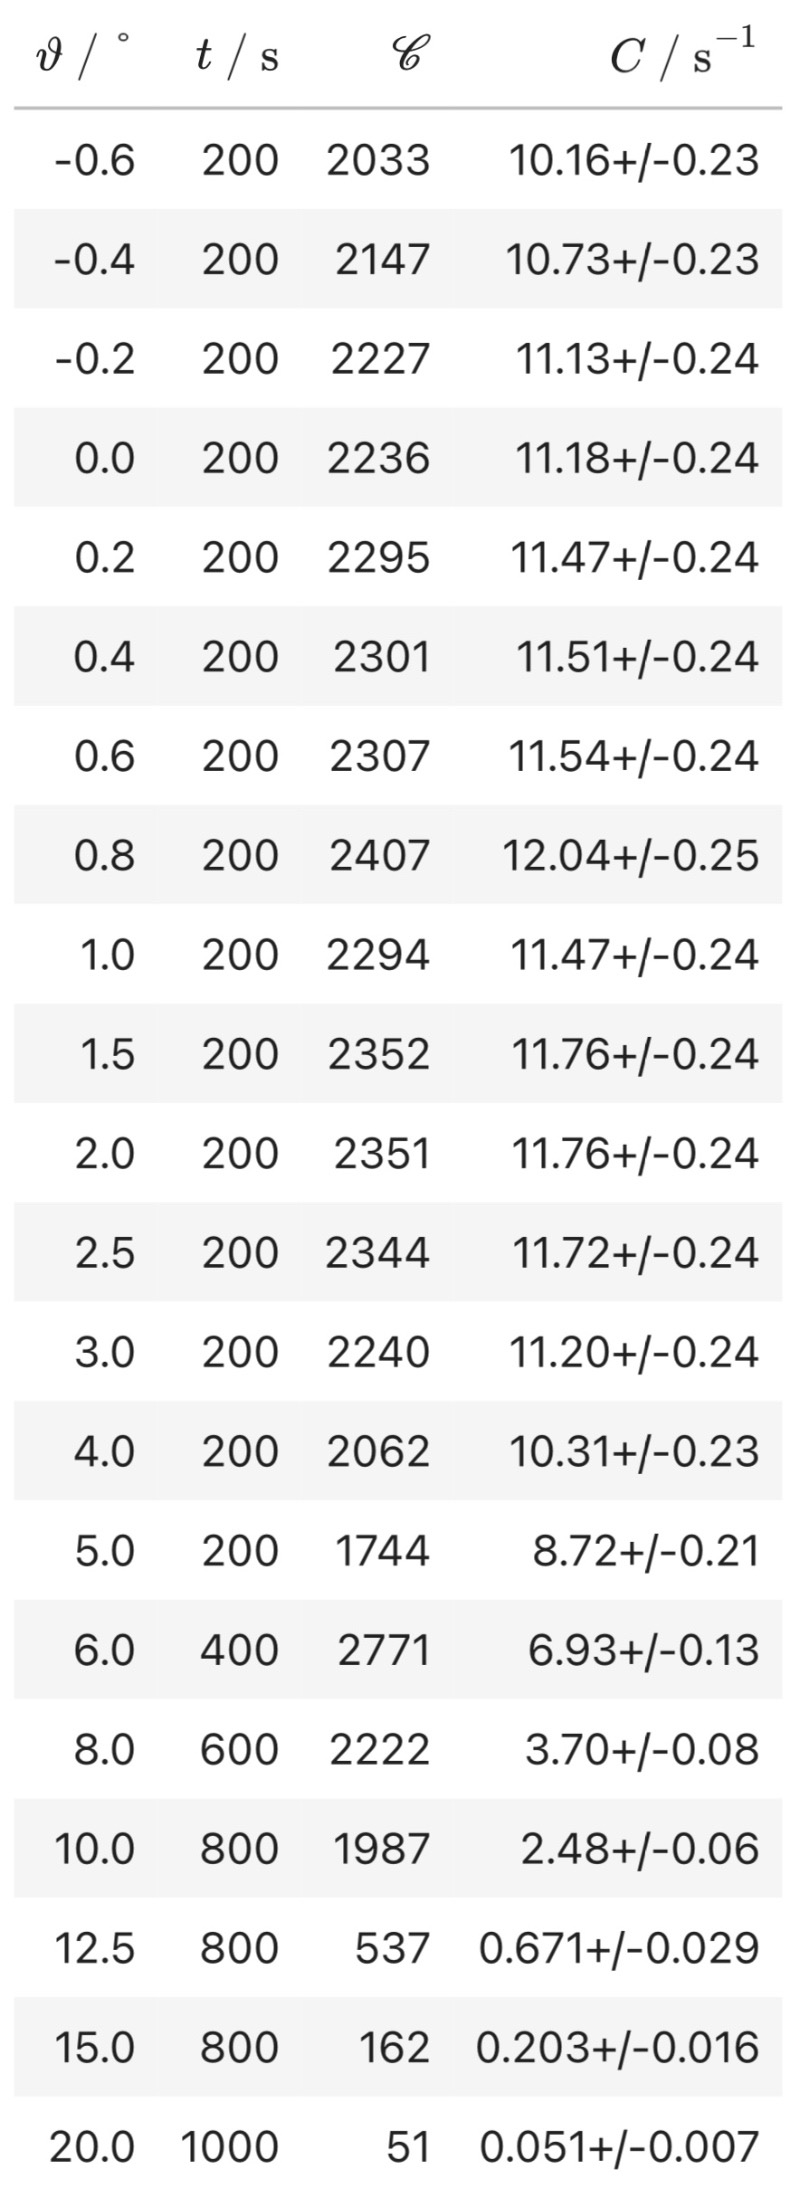
\includegraphics[width=0.32\textwidth]{content/tabelle/Streuwinkel.jpg}
    \label{tab:Streuwinkel}
\end{table}

\begin{figure}[H]
    \centering
    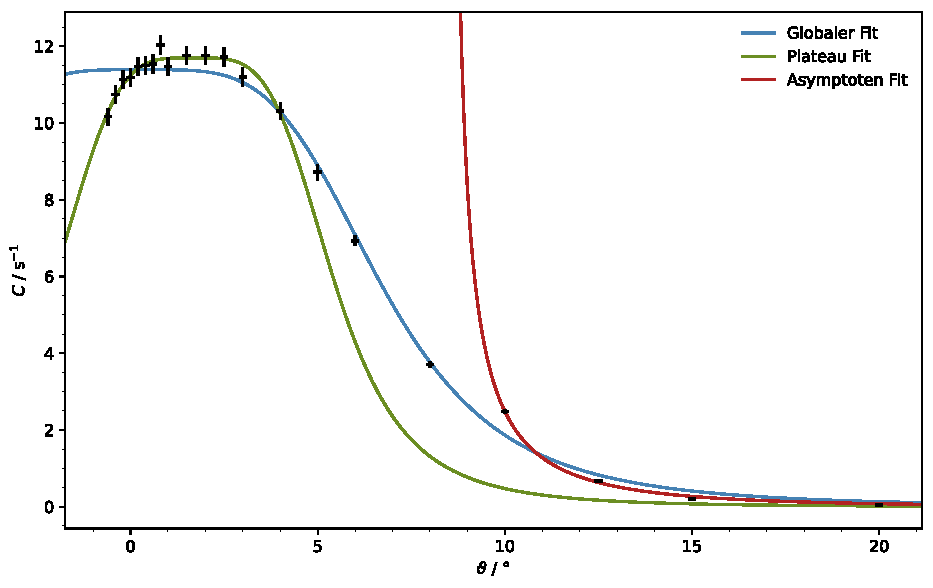
\includegraphics[width=\textwidth]{content/messung/Streuwinkel.pdf}
    \caption{Streuwinkelabhängigkeit der Zählrate.}
    \label{fig:Streuwinkel}
\end{figure}
